\documentclass[11pt]{article}
\usepackage{parskip}
\usepackage[margin=3.5cm]{geometry}
\usepackage{amsmath}
\usepackage{amssymb}
\usepackage[shortlabels]{enumitem}
\usepackage{fancyhdr}
\usepackage{gensymb} %for degree symbol
\usepackage{graphicx} %to add figures to the document
\usepackage{subfigure} %used for side by side figures
\usepackage{url} %used for urls
\usepackage[nottoc, numbib]{tocbibind} %include references in toc
\usepackage[toc,page]{appendix} %used for appendix
\usepackage{listings} % used for R code
\usepackage{multirow} % multirows for tables
\usepackage{array}	% vertically centre contents in table cells
\usepackage{imakeidx} %add index
\usepackage{algorithm}
\usepackage{algpseudocode}
\usepackage[table,xcdraw]{xcolor}
%\usepackage[boxruled, dotocloa]{algorithm2e} %pretty pseudocode
\lstset{language=R, basicstyle=\ttfamily} % To add R code in appendix
\graphicspath{ {C:/Users/Gemma/Documents/UNISA/Honours/Project 2017/02 Preliminary Report/} } %folder name where images are contained in the current directory
\DeclareMathSymbol{,}{0}{letters}{"3B}
\DeclareMathOperator{\argh}{argh}
\DeclareMathOperator*{\nut}{Nut}
\newcommand{\np}{\newpage}
\indexsetup{level=\section}
\makeindex[name=terms,title=Index of Terms,columns=2]
\makeindex[name=authors,title=Index of Authors,columns=2]	%initiate the index
\setcounter{page}{1}
\pagestyle{fancy}
\fancyhf{}
\rhead{Assignment 2: Preliminary Report\\ HONPR2C}
\lhead{Gemma Dawson\\ Student Number: 50223909}
\cfoot{\thepage}


\begin{document}

	\title{
		\begin{figure}[!htb]
			\begin{center}
				
\includegraphics[width=12cm]{unisa.png}
			\end{center}
		\end{figure}
		Department of Decision Sciences\\[3mm]
		HONPR2C\\
		Project II \\[2cm]		
		{\Huge \textbf{An analysis of heuristics for the \emph{p}-median problem}}\\[15mm]
		Assignment 2: Preliminary Report\\[3mm]
		Assignment Unique Number: 650898\\[2cm]
	}
	\author{\textbf{\Large Gemma Dawson}\\[3mm]
		\textbf{\Large 50223909}\\[3mm]
		\textbf{Study Leader: Ms J L le Roux}
	}
	\date{\Large 30 August 2017}	
	\maketitle
	\thispagestyle{empty}
	\np
	
	\section*{Signed Declaration}
	I hereby declare that this project is my own work and that all the sources that I have used or quoted have been indicated and acknowledged by means of complete references.
	
	Signed:
	\begin{figure}[!htb]
			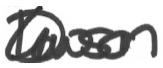
\includegraphics[width=3cm]{signature.png}
	\end{figure}

	Gemma Dawson\\
	Student Number: 50223909\\
	
	
	\thispagestyle{empty}
	\np
	
	\tableofcontents
	\thispagestyle{empty}
	\np

\setcounter{page}{1}		
	\section{Introduction} \label{introduction}
	The network facility location problem of finding a location for facilities or public services within a given space by optimising some predefined objective, is not a simple one.  Within the single-objective branch of network location problems, there is a plethora of papers exploring minisum, minimax, and covering problems.
	
	If the number of facilities needed is known, and these facilities need to be located in the manner of minimising the total distance between demand nodes and their assigned facility, then the decision-maker is facing a \emph{p}-median problem.
	
	The \emph{p}-median problem \index[terms]{p-median problem} is well studied and many different approaches to finding both exact and approximate solutions have been proposed, but determining which method would be best for a particular problem is not clear.
	
	This study will analyse and compare several heuristics applied to the \emph{p}-median problem in the hope that this decision may be made more clear.	
	
	
	\section{Description of the Problem} \label{problem.statement}
	The uncapacitated \emph{p}-median problem has been widely studied and many different approaches to finding an acceptable, if not optimal, solution have been presented over the past fifty years.
	
	The focus of this study is to statistically analyse and compare the results obtained from various heuristic\index[terms]{heuristic} and metaheuristic\index[terms]{metaheuristic} algorithms applied to the \emph{p}-median problem\index[terms]{p-median problem}.
	
	Different heuristics applied to \emph{p}-median problems can produce varying quality of results dependant on the size of the original problem.  As algorithms\index[terms]{algorithm} take a considerable amount of time and research to be suitably set-up and run, it may be of benefit to have some prior knowledge of which heuristics may be suitable for the problem on hand.
	
	As such, the main objective of this study would be to provide an indication of which method would be best suited to a given problem.
	
	This study will also investigate the computational time each algorithm requires to generate a solution, taking into account the size of the problem being solved.
	
	Since parametrisation of heuristics play a crucial part of the efficiency of the algorithm and the quality of the results it produces, this will be explained in detail in the study.  Given time, different approaches to the same heuristic may be explored as well.	
	
	
	\section{Literature Study} \label{lit.study}
	While the \emph{p}-median problem\index{p-median problem} may have been tackled by academics before 1964, it was first formally defined and formulated by Hakimi\index[authors]{Hakimi, S.} \cite{HAKI64}.  It was also in this paper that Hakimi\index[authors]{Hakimi, S.} proved that the optimal location of a facility in a connected discrete network would always be found to correspond to the location of a demand node.  This considerably reduces the solution search space.
	
	A few years later, ReVelle\index[authors]{ReVelle, C.} and Swain \index[authors]{Swain, R.}\cite{REVE70} formulated the \emph{p}-median problem as an integer programme \index[terms]{integer programme} which provided the answers to both the question of where the optimal medians were located as well as which demand nodes should be allocated to each median.  In this paper, the solution properties of solving this problem with linear programming \index[terms]{linear programming} using the branch-and-bound technique \index[terms]{linear programme!branch-and-bound} was also discussed.
	
	Later that decade, it was shown that the \emph{p}-median problem is NP-hard \index[terms]{NP-hard} and as such there exists no algorithm that can find the optimal solution within polynomial time.  Since most real-world problems are very large in nature, this poses a great problem.  Well developed heuristics\index[terms]{heuristic} can provide satisfactory solutions and many such approaches have been proposed.  Mladenovi\'{c}\index[authors]{Mladenovi\'{c}, N.} et al. \cite{MLAD07} produced a comprehensive survey of the heuristics that have been used to solve the \emph{p}-median problem.  This survey divides heuristics into two groups, Classical Heuristics and Metaheuristics\index[terms]{metaheuristic}.  The classical heuristics group consists of constructive heuristics\index[terms]{heuristic!constructive}, such as the greedy algorithm\index[terms]{greedy algorithm}\index[terms]{heuristic!greedy algorithm}, local search\index[terms]{local search}\index[terms]{heuristic!local search}, and mathematical programming\index[terms]{mathematical programming}.  The metaheuristics group lists tabu search\index[terms]{tabu search}\index[terms]{metaheuristic!tabu search}, variable neighbourhood search\index[terms]{variable neighbourhood search}\index[terms]{metaheuristic!variable neighbourhood search}, and simulated annealing\index[terms]{simulated annealing}\index[terms]{metaheuristic!simulated annealing} among others.
	
	There do exist studies that analysis the efficiency of heuristics in solving the \emph{p}-median.  Simulated annealing\index{simulated annealing}\index[terms]{metaheuristic!simulated annealing} was analysed by Chiyoshi\index[authors]{Chiyoshi, F.}  and Galv\~{a}o \index[authors]{Galv\~{a}o, R.} \cite{CHIY00} while Alp\index[authors]{Alp, O.} et al. \cite{ALPO03} investigated their proposed genetic algorithm\index{genetic algorithm}.  Hansen\index{Hansen, P.} and Mladenovi\'{c}\index[authors]{Mladenovi\'{c}, N.} \cite{HANS01} applied the variable neighbourhood search algorithm\index[terms]{variable neighbourhood search}\index[terms]{metaheuristic!variable neighbourhood search} to the \emph{p}-median problem as well as heuristic concentration\index[terms]{heuristic concentration}, tabu search\index[terms]{tabu search}\index[terms]{metaheuristic!tabu search}, and the greedy interchange algorithm\index[terms]{greedy interchange algorithm}.  These studies used Beasley's test problem dataset\index[terms]{Beasley's test problem dataset} although Hansen\index[authors]{Hansen, P.}  and Mladenovi\'{c}'s\index[authors]{Mladenovi\'{c}, N.} review only used a portion of the available test problems.  
	
	Rolland\index[authors]{Rolland, E.} et al. \cite{ROLL97} explored the efficiency of tabu search\index[terms]{tabu search}\index[terms]{metaheuristic!tabu search} using randomly generated datasets as test problems, and this was compared to results obtained from a two-exchange heuristic\index[terms]{heuristic} and an integer programming\index[terms]{integer programming} algorithm.  A heuristic\index[terms]{heuristic} concentration was compared to tabu search by Rosing\index[authors]{Rosing, K. E.} et al. \cite{ROSI98}.  Since datasets were independently and randomly generated for each of these studies, it makes it very difficult to compare results.
	
	
	\section{Methodology} \label{methodology}
	All algorithms have been coded in R\index[terms]{R (programming language)} \cite{RPROGRAMME}, an open source programming language, due to its ease of use, extensive availability of online resources as well as the functionality provided by downloadable packages that provide useful data handling and visualisation.
	
	As the results of the algorithms\index[terms]{algorithm} under investigation are to be compared, identical problems have been presented to each algorithm to solve.  Beasley \cite{BEAS90} \index[authors]{Beasley, J.} offers a forty-instance dataset\index[terms]{Beasley's test problem dataset} which comprises of problems ranging from 100 to 900 demand nodes that require the locations of between five and 200 medians to be determined.  These datasets are given in a text format presenting the pairs of nodes along with the associated cost of traversing this node pair.  These text files were converted to cost matrices using the R package igraph \cite{RIGRAPH}.  These matrices provide the cost of travel from one node to any other node in each network of the forty instances.
	
	Beasley's library also provides the optimal solution's weighted total cost objective function value for each of the forty instances in the dataset.  This allows the results obtained from the algorithms to be objectively assessed against the optimal solution.  
	
	As all algorithms require nodes associated with an the minimum cost to be identified, a function in R \index[terms]{R (programming language)} was written to deal with the issue when more than one nodes offer the same minimum cost.  R's base package offers a minimum function, but if more than one element in the vector that is passed to this function equals the minimum value, only the first of such elements will be returned and all subsequent elements will be ignored.  However, the new function will return a randomly selected element.  A direct consequence of introducing this element of randomness is that an algorithm may produce different results and as such, for every problem in the forty-instance dataset, each algorithm will be run 100 times and the resulting objective function value was recorded, which allowed the deviation of each algorithm's solution from the optimal solution to be analysed.  In addition, the computational time required for each of the 100 runs was timed.
	
		
	\section{Classical Heuristics and Metaheuristics} \label{classical.meta.heuristics}
	\subsection{Overview} \label{heuristics.overview}
	As previously mentioned, a review of approaches to solving the \textit{p}-median problem\index[terms]{p-median} was presented by Mladenovi\'{c}\index[authors]{Mladenovi\'{c}, N.} et al. \cite{MLAD07} in 2007.  This paper divided heuristics\index[terms]{heuristic} into one of two groups, Classical Heuristics\index[terms]{heuristic!classical heuristic} and Metaheuristics\index[terms]{heuristic!metaheuristic}.  This classification has been utilised in this study.
	
	An algorithm can be classified as a Classical Heuristic if it is developed for the purpose of solving the \emph{p}-median problem, while a heuristic that was developed independent of the \emph{p}-median problem can be termed a Metaheuristic.
		
	
	\subsection{Pseudocode Notation} \label{pseudocode.notation}
	For each algorithm examined in this study, a pseudocode will be presented using notation given below.  This notation is similar to that used by Whitaker \index[authors]{Whitaker, R.}\cite{WHIT83}.
	\begin{align*}
	G &: \text{the problem network}\\
	n &: \text{the number of nodes within the network}\\
	m &: \text{the number of nodes nodes that are available to be assigned as a median}\\
	p &: \text{the number of medians required by the solution}\\
	M &: \text{the set of nodes that are available to be assigned as a median}\\
	P^{*} &: \text{the set of medians where } P^{*} \subset M\\
	P &: \text{the set of free nodes not in the solution median set where } P \subset M\\
			& \quad \text{ and } P \cup P^{*} = M\\
	S^{*} &: \text{objective function value for supplying the network } G\\
	k &: \text{an iteration parameter}\\
	\infty &: \text{an arbitrarily large number}\\
	d_{ij} &: \text{the cost of travelling from node \emph{i} to potential median \emph{j}}\\
	u_{i}^{k} &: \text{the cost of travelling from node \emph{i} to the closest median \emph{j}}\\
			& \quad \text{ where } j \in P^{*} \text{ during iteration } k\\
	w_{i}^{k} &: \text{the cost of travelling from node \emph{i} to the second closest median}\\
			& \quad \text{\emph{j} where } j \in P^{*} \text{ during iteration } k\\
	c_{j}^{k} &: \text{the potential value of \emph{S*} if node \emph{j} is added to the median set \emph{P*} during}\\
			& \quad \text{ iteration \emph{k}}\\
	S_{r} &: \text{the value of \emph{S*} after adding node \emph{r} to the median set \emph{P*}}\\
	S_{rt} &: \text{the potential change to S* resulting from the interchange of node \emph{r} with}\\
		& \quad \text{median \emph{t}}\\
	S^k &: \text{the change in the value of $S^*$ during iteration $k$}\\
	I \text{, } J \text{, } K_{j} &: \text{subsets of the \emph{n} nodes defined as needed in the pseudocode}\\
	a \text{, } b \text{, } z \text{, } q &: \text{indices and parameters defined as needed in the pseudocode}\\
	\emptyset &: \text{an empty set}	
	\end{align*}
	

	\section{Classical Heuristics: Constructive} \label{classicheuristics.constructive}
	A constructive heuristic\index[terms]{constructive heuristic}\index[terms]{heuristic!constructive} is a technique that starts with an empty solution and each iteration extends this solution until a complete solution has been found.  Within the context of the unconstrained \emph{p}-median problem, for each iteration of the algorithm, a median is identified by some deterministic method and added to the current solution.  This process continues until the median set contains \emph{p} elements.
	
	\subsection{The Greedy Algorithm}\label{greedyalgo}
	The greedy algorithm,\index[terms]{greedy algorithm}\index[terms]{heuristic!greedy algorithm} as described by Whitaker \cite{WHIT83}, \index[author]{Whitaker, R.} is a simple recursive algorithm that starts with an empty median set and, with each iteration of the algorithm, adds a node to the median set.  The node that is added to the median set is the one that decreases the objective function value the most when compared to the other non-median nodes.
	
	\subsubsection{Pseudocode}
	\index[terms]{greedy algorithm! pseudocode} 	
	\begin{algorithm}
		\caption{Greedy Algorithm}
		\begin{algorithmic}[0]
			
			\Statex 
			\Statex INPUT: Cost Matrix
						
			\Statex
			\Statex STEP 0: Initialisation	
			\begin{equation*}
			\text{Set } P^{*} = \emptyset \text{; } k = 1\text{; and }u_i^1 = \infty\text{ for all } i=1,2,\dots,n
			\end{equation*}
			
			\Statex 
			\Statex STEP 1: For each free node, the objective function value resulting from selecting this node as a median is determined.  This objective function value is calculated by summing the cost of travel for each node in the network to either the closest median or the free node under investigation, whichever is smallest.
			\begin{equation*}
			c_j^k = \sum_{i=1}^{n}\min(d_{ij} \text{, } u_i^k) \quad \forall j \in M \text{, } j \notin P^*
			\end{equation*}
			
			\Statex 
			\Statex STEP 2: The free node that will result in the smallest possible objective function value is identified, and the objective function value is updated.
			\begin{equation*}
			S_r = \min_{j \notin P*}(c_j^k) \quad \text{for } r \in M \text{, } r \notin P^*
			\end{equation*}
			
			\Statex 
			\Statex STEP 3: Add node \emph{r} to the set of medians and then determine if the algorithm has completed the number of required iterations.
			\begin{equation*}
			P^* = P^* \cup r
			\end{equation*}
			
			\If{$k = p$}
			\Statex go to STEP 5
			[
			\Else
			\Statex go to STEP 4
			]
			\EndIf
			
\Statex	

\algstore{greedy}
\end{algorithmic}
\end{algorithm}

\begin{algorithm}
%\caption{Greedy Algorithm (continued)}
\begin{algorithmic}[0]
\algrestore{greedy}
			
			\Statex 
			\Statex STEP 4: Increase the value of iteration parameter and update the cost of travelling from any node to its closet median given that node $r$ has been added to the median set.
			\begin{align*}
			k &= k+1\\
			u_i^k &= \min(d_{ir} \text{, } u_i^{k-1}) \quad \text{for } i = 1,2,3 \dots,n
			\end{align*}
			\Statex \begin{center} Go to STEP 1 \end{center}
			
			\Statex 
			\Statex STEP 5: Once \emph{p} iterations are complete, set the final objective function value equal to the current iteration's objective function value and stop the algorithm.
			\begin{center}
				$S^{*} = S_r$ and STOP
			\end{center}
			
			
		\end{algorithmic}
	\end{algorithm}

	
	
	\subsection{The Fast Greedy Algorithm} \label{fastgreedyalgo}
	Whitaker \cite{WHIT83} \index[authors]{Whitaker, R.} proposed the fast greedy algorithm.\index[terms]{heuristic!fast greedy algorithm}\index[terms]{constructive heuristic!fast greedy algorithm}\index[terms]{fast greedy algorithm} This algorithm differs from the greedy algorithm in that only the nodes that were re-assigned to a new median in the preceding iteration are investigated.  From these nodes, the new median is determined to be the one that will maximise the decrease in the objective function value.
	
	\subsubsection{Pseudocode}
	\index[terms]{fast greedy algorithm! pseudocode} 	
	\begin{algorithm}
		\caption{Fast Greedy Algorithm}
		\begin{algorithmic}[0]
			
			\Statex 
			\Statex INPUT: Cost Matrix
						
			\Statex
			\Statex STEP 0: Initialisation 	
			\begin{align*}
			\text{Set } & P^{*} = \emptyset \text{; } I = \emptyset \text{; } k = 1\\
			& c_j^0=c_j^1 = 0 \text{ for }j\in M\\
			& u_i^0 = 0 \text{; } u_i^1 = \infty\text{ for all } i=1,2,\dots,n\\
			& I=I\cup i \text{ for } i=1,2,\dots,n
			\end{align*}
\Statex	
\algstore{bkbreak}
\end{algorithmic}
\end{algorithm}

\begin{algorithm}
%\caption{Greedy Algorithm (continued)}
\begin{algorithmic}[0]
\algrestore{bkbreak}
			
			\Statex
			\Statex STEP 1: For each free node that was reassigned to a new median in the previous iteration, the objective function value resulting from selecting this node as a median is determined.  This objective function value is calculated by summing the cost of travel for each node in the network to either the closest median or the free node under investigation, whichever is smallest.  For the first iteration, all nodes in the network are considered part of the reassigned set.
			\begin{equation*}
			c_j^k = \sum_{i\in I}\min(d_{ij} \text{, } u_i^k) + c_j^{k-1} - \sum_{i\in I}\min(d_{ij} \text{, } u_i^{k-1})\quad \forall j \in M \text{, } j \notin P^*
			\end{equation*}

			
			\Statex
			\Statex STEP 2: The free node that will result in the smallest possible objective function value is identified, and the objective function value is updated.
			\begin{equation*}
			S_r = \min_{j \notin P*}(c_j^k) \quad \text{for } r \in M \text{, } r \notin P^*
			\end{equation*}
			
			\Statex
			\Statex STEP 3: Add node \emph{r} to the set of medians and then determine if the algorithm has completed the number of required iterations.
			\begin{equation*}
			P^* = P^* \cup r
			\end{equation*}
			
			\If{$k = p$}
			\Statex go to STEP 5
			[
			\Else
			\Statex Set $I = \emptyset$ and go to STEP 4
			]
			\EndIf
			
			
			\Statex
			\Statex STEP 4: Increase the value of iteration parameter and update the cost of travelling from any node to its closet median given that node $r$ has been added to the median set.
			\begin{align*}
			k &= k+1\\
			u_i^k &= \min(d_{ir} \text{, } u_i^{k-1}) \quad \text{for } i = 1,2,3 \dots,n\\
			\end{align*}
			
			\If{$d_{ir}<u_i^{k-1}$}
			[
			\Statex $I=I\cup i$
			\Statex go to STEP 1]
			\EndIf
			
			\Statex
			\Statex STEP 5: Once \emph{p} iterations are complete, set the final objective function value equal to the current iteration's objective function value and stop the algorithm.
			\begin{center}
				$S^{*} = S_r$ and STOP
			\end{center}
			
		\end{algorithmic}
	\end{algorithm}


\np
	\subsection{The Stingy Algorithm} \label{stingyalgo}
	The stingy algorithm was suggested by Feldman, \index[author]{Feldman, E.} Lehrer, \index[author]{Lehrer, F.} and Ray \index[author]{Ray, T.} in their paper \cite{FELD66} published in 1966.  
	Instead of starting with an empty median set and recursively adding a node until all \textit{p} medians are assigned, the stingy algorithm\index[terms]{heuristic!stingy algorithm}\index[terms]{stingy algorithm}\index[terms]{constructive heuristic!stingy algorithm} begins with all nodes in the network being designated as a median.  Nodes are removed one at a time until only required \textit{p} medians remain in the median set.
	
	\subsubsection{Pseudocode}
	\index[terms]{stingy algorithm! pseudocode} 
	\begin{algorithm}
		\caption{Stingy Algorithm}
		\begin{algorithmic}[0]
			
			
			\Statex 
			\Statex INPUT: Cost Matrix
			
			
			\Statex 
			\Statex STEP 0: Initialisation 	
			\begin{equation*}
			\text{Set } P^*=M \text{; } P=\emptyset \text{ and } u_i=0 \text{ for all } i=1,2,\dots,n
			\end{equation*}
			
			\Statex 
			\Statex STEP 1: For each node that belongs to the median set, find the value of the objective function if this node were to be removed from the median set.
			\begin{equation*}
			c_j^* = \sum_{i=1}^{n} \min_{j\in P^*, j\neq i} d_{ij}
			\end{equation*}
			
			\Statex 
			\Statex STEP 2: Identify which node results in the smallest possible objective function value.
			\Statex Find node $r$ such that 
			\begin{equation*}
			S_r = \min_{j \in P*}(c_j^k) \quad \text{for } r \in P^* \text{, } r \notin P
			\end{equation*}
			
			
			\Statex 
			\Statex STEP 3: Remove this node from the set of medians.
			\begin{align*}
			P^* &= P^* \backslash \{r\} & P &= P \cup \{r\}
			\end{align*}
			
			\Statex 
			\Statex STEP 4: Update the iteration parameter.
			\begin{equation*}
			k = k+1
			\end{equation*}
			
			
			\Statex 
			\Statex STEP 5: Once \emph{p} iterations are complete, set the final objective function value equal to the current iteration's objective function value and stop the algorithm.
			\begin{center}
				$S^{*} = S_r$ and STOP
			\end{center}
			
			
		\end{algorithmic}
	\end{algorithm}

	
	\subsection{Computational Results} \label{classicheuristics.constructive.results}
	The average solution accuracy for each of the forty test problems from both the greedy algorithm\index[terms]{greedy algorithm}\index[terms]{greedy algorithm! results}\index[terms]{constructive heuristic!greedy algorithm}\index[terms]{heuristic!greedy algorithm} and the fast greedy algorithm\index[terms]{fast greedy algorithm! results}\index[terms]{fast greedy algorithm}\index[terms]{constructive heuristic!fast greedy algorithm}\index[terms]{heuristic!fast greedy algorithm} as well as the average computational time can be seen in table \ref{CH.Results.table}.  
	
	Figure \ref{CH.av.acc} shows the average accuracy of the solution's objective function value for each of the forty test problems.  It can be seen that the greedy algorithm was able to produce results that were very close to the optimal value with slight decreases as the number of medians required increased.  In table \ref{CH.Results.table}, you can see that all the average objective function value was at most 4\% less than the optimal objective function value.
	
	The fast greedy algorithm produced results for about twenty problems that were 50\% worse than the true optimal.  The test problems with the highest accuracy rate when using the fast greedy correspond to the test problems that demanded five medians.  The massive difference in accuracy for the fast greedy algorithm is clearly visible in figure \ref{CH.av.acc} and as such the code for this algorithm needs to be reviewed.
	
	\begin{figure}[H]
		\begin{center}
			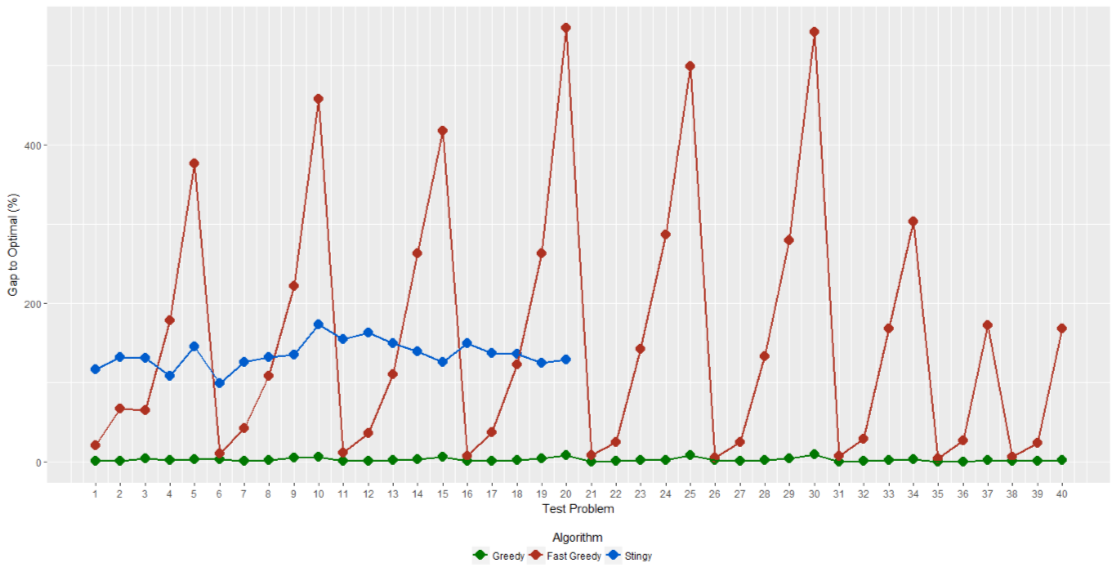
\includegraphics[width=14cm]{CHavacc.png}
			\caption{Average Solution Accuracy per Test Problem}
			\label{CH.av.acc}
		\end{center}
	\end{figure}

	In figure \ref{CH.av.time}, the average computational time for both the greedy algorithm\index[terms]{greedy algorithm}\index[terms]{greedy algorithm! results}\index[terms]{constructive heuristic!greedy algorithm}\index[terms]{heuristic!greedy algorithm} and the fast greedy algorithm\index[terms]{fast greedy algorithm}\index[terms]{fast greedy algorithm! results}\index[terms]{constructive heuristic!fast greedy algorithm}\index[terms]{heuristic!fast greedy algorithm} increases as the number of medians demanded by the test problem increases.  It can be seen in figure \ref{CH.av.time} that the fast greedy algorithm takes longer than the greedy algorithm for every test problem.
	
	\begin{figure}[H]
		\begin{center}
			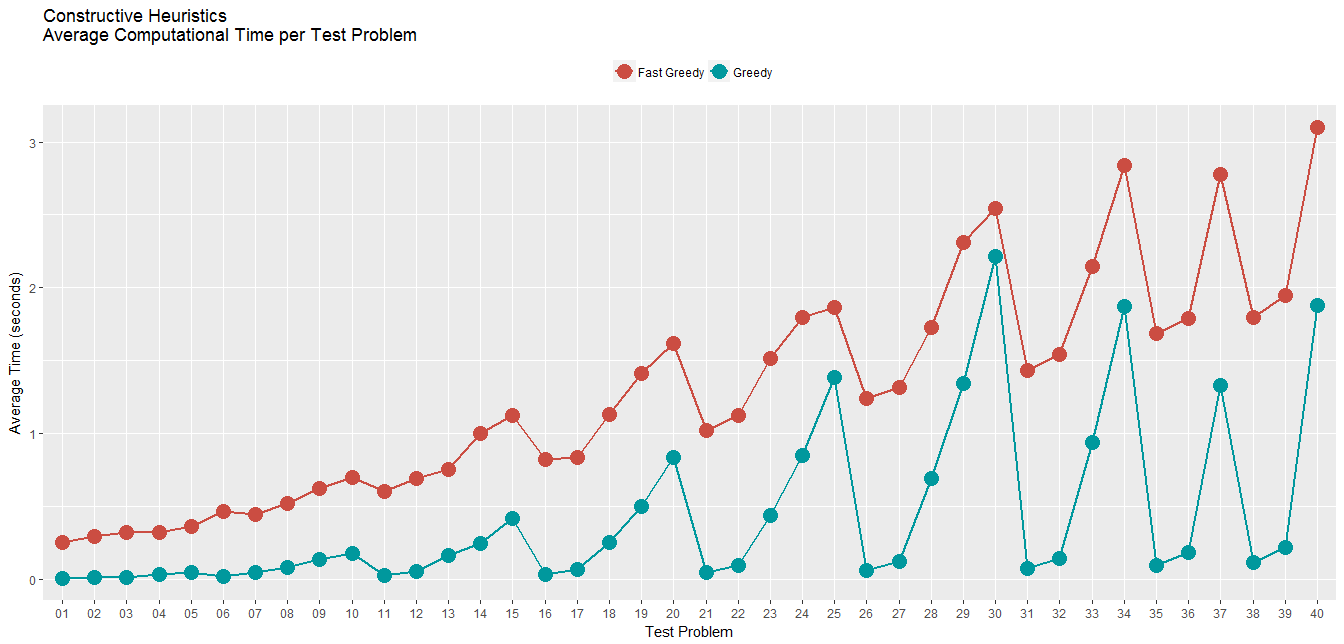
\includegraphics[width=14cm]{CHavtime.png}
			\caption{Average Computational Time per Test Problem}
			\label{CH.av.time}
		\end{center}
	\end{figure}

	Figures \ref{greedymediantime} and \ref{fastgreedymediantime} show the number of medians demanded by a test problem against the average computational time for the greedy algorithm and the fast greedy algorithm respectively.  For the nine test problems with $p=5$, the greedy algorithm produces a solution between 0.01 and 0.12 seconds where the increase in time can be attributed to the number of nodes in the network and this relatively small increase in time can be seen in figure \ref{greedymediantime}.  As the network size increases, so does the spread between the average computational time required by the greedy algorithm to return a solution.    

	\begin{figure}[H]
		\begin{center}
			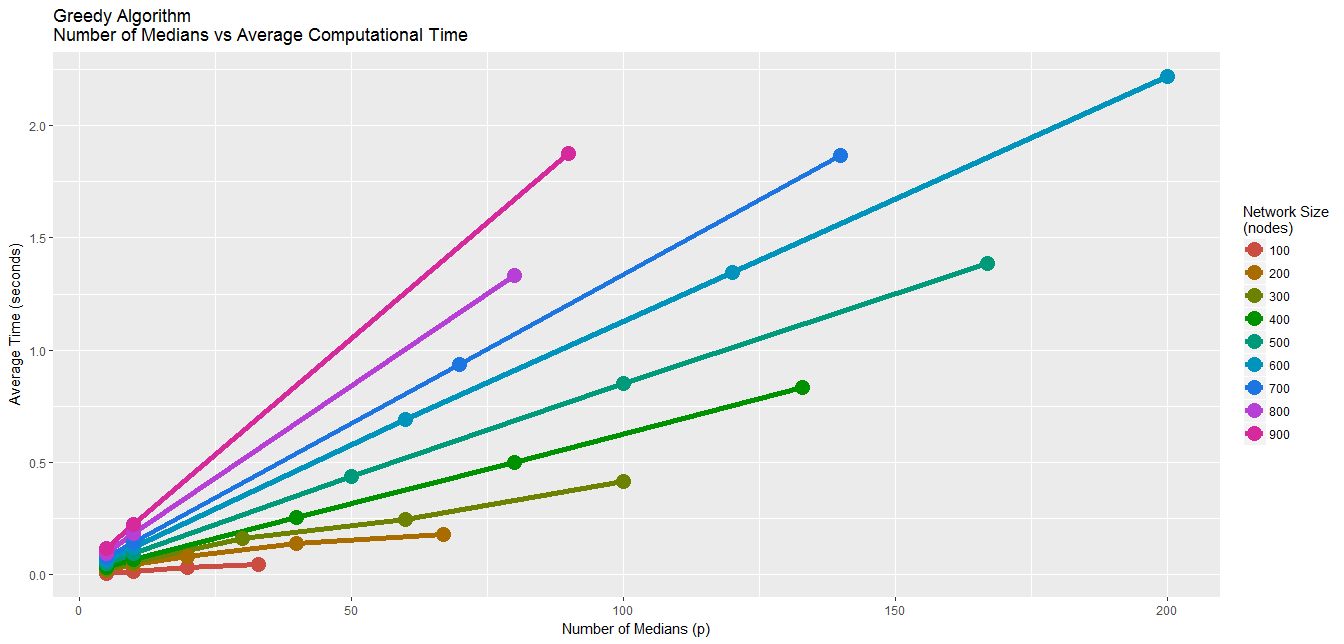
\includegraphics[width=15cm]{Greedy.png}
			\caption{Greedy Algorithm}
			\label{greedymediantime}
		\end{center}
	\end{figure}
	
	It can be seen in figure \ref{fastgreedymediantime} that the fast greedy algorithm has not lived up to its name.  The average time taken to produce results for the $p=5$ test problems was between 0.26 and 1.79 seconds.  This spread can be seen in figure \ref{fastgreedymediantime} and can be attributed to the size of the network.  This may be due to the additional step of identifying the nodes that were reassigned to a new median in the previous iteration.  The design of the fast greedy algorithm's code needs to be reviewed to determine if the full power of R is being exploited.  The algorithmic complexity of both the greedy algorithm and the fast greedy algorithm \index[terms]{fast greedy algorithm}\index[terms]{fast greedy algorithm! results}\index[terms]{constructive heuristic!fast greedy algorithm}\index[terms]{heuristic!fast greedy algorithm} need to be evaluated in order to determine if it is possible for this algorithm to be faster than the greedy algorithm. \index[terms]{greedy algorithm}\index[terms]{greedy algorithm! results}\index[terms]{constructive heuristic!greedy algorithm}\index[terms]{heuristic!greedy algorithm}

	\begin{figure}[H]
		\begin{center}
		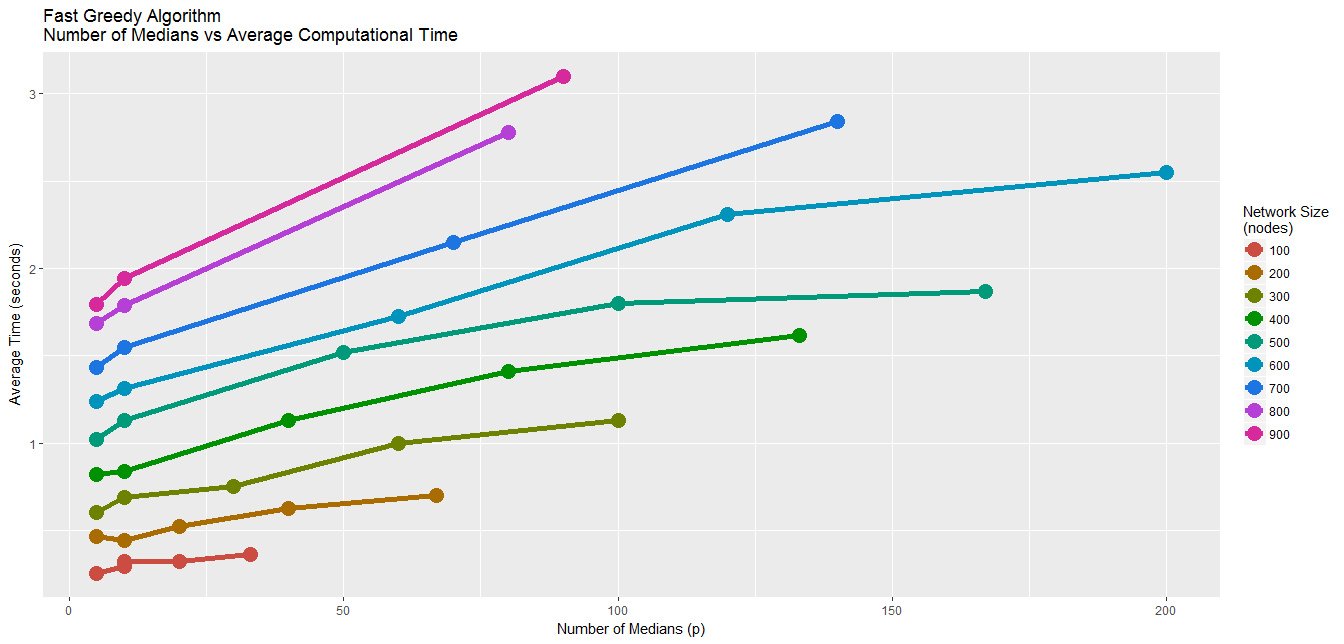
\includegraphics[width=15cm]{FastGreedy.png}
			\caption{Fast Greedy Algorithm}
			\label{fastgreedymediantime}
		\end{center}
	\end{figure}


	Based on the work done by Whitaker \cite{WHIT83}, \index[author]{Whitaker, R.} it was expected that the fast greedy algorithm\index[terms]{fast greedy algorithm}\index[terms]{fast greedy algorithm! results}\index[terms]{constructive heuristic!fast greedy algorithm}\index[terms]{heuristic!fast greedy algorithm} would produce results quicker than the greedy algorithm.  The trade-off in finding a solution faster would be an objective function value that is less accurate when compared to the optimal objective function value.  The substantial drop in accuracy as the number of medians demanded increases is far too large to accept, even if the algorithm were producing results faster than the greedy algorithm.
	
	The code for the stingy algorithm has been completed, but still needs to be thoroughly reviewed before running the 100 iterations for each of the forty test problems.  Once this has been completed, the results along with the computational time will be included in the final report of this study.  These results will also be analysed and compared to both the greedy algorithm and the fast greedy algorithm.  The expectation is that this algorithm will take longer to run for the small median problems, but for test problems requiring a large number of medians, the computational time may be comparable.  
	
	\begin{table}[]
		\centering
		\caption{Constructive Heuristic Results}
		\label{CH.Results.table} \index[terms]{greedy algorithm}\index[terms]{greedy algorithm! results}\index[terms]{constructive heuristic!greedy algorithm}\index[terms]{heuristic!greedy algorithm}
		\index[terms]{fast greedy algorithm}\index[terms]{fast greedy algorithm! results}\index[terms]{constructive heuristic!fast greedy algorithm}\index[terms]{heuristic!fast greedy algorithm}
		\begin{tabular}{ccccccc}
			\hline
			&  &  & \multicolumn{2}{c}{\textbf{GREEDY}} & \multicolumn{2}{c}{\textbf{FAST GREEDY}} \\ \cline{4-7} 
			\multirow{-2}{*}{\textbf{\begin{tabular}[c]{@{}c@{}}\small{Test} \\ \small{Problem}\end{tabular}}} & \multirow{-2}{*}{\textbf{\begin{tabular}[c]{@{}c@{}}\small{Medians} \\ \small{(p)}\end{tabular}}} & \multirow{-2}{*}{\textbf{\begin{tabular}[c]{@{}c@{}}\small{Network} \\ \small{(nodes)}\end{tabular}}} & \textbf{\begin{tabular}[c]{@{}c@{}}\small{Av. Sol.}\\ \small{Accuracy}\end{tabular}} & \textbf{\begin{tabular}[c]{@{}c@{}}\small{Av. Comp.} \\ \small{Time (sec)}\end{tabular}} & \textbf{\begin{tabular}[c]{@{}c@{}}\small{Av. Sol.}\\ \small{Accuracy}\end{tabular}} & \textbf{\begin{tabular}[c]{@{}c@{}}\small{Av. Comp.}\\ \small{Time (sec)}\end{tabular}} \\ \hline
			\rowcolor[HTML]{EFEFEF} 
			01 & 5 & 100 & 0.99 & 0.01 & 0.83 & 0.26 \\ 
			\rowcolor[HTML]{EFEFEF} 
			02 & 10 & 100 & 0.99 & 0.02 & 0.60 & 0.29 \\ 
			\rowcolor[HTML]{EFEFEF} 
			03 & 10 & 100 & 0.97 & 0.02 & 0.61 & 0.32 \\ 
			\rowcolor[HTML]{EFEFEF} 
			04 & 20 & 100 & 0.98 & 0.03 & 0.36 & 0.32 \\
			\rowcolor[HTML]{EFEFEF} 
			05 & 33 & 100 & 0.98 & 0.05 & 0.21 & 0.36 \\
			06 & 5 & 200 & 0.97 & 0.02 & 0.91 & 0.47 \\ 
			07 & 10 & 200 & 1.00 & 0.05 & 0.71 & 0.44 \\
			08 & 20 & 200 & 0.99 & 0.08 & 0.48 & 0.52 \\
			09 & 40 & 200 & 0.96 & 0.14 & 0.31 & 0.63 \\
			10 & 67 & 200 & 0.97 & 0.18 & 0.18 & 0.70 \\
			\rowcolor[HTML]{EFEFEF} 
			11 & 5 & 300 & 1.00 & 0.03 & 0.90 & 0.61 \\ 
			\rowcolor[HTML]{EFEFEF} 
			12 & 10 & 300 & 1.00 & 0.06 & 0.73 & 0.69 \\ 
			\rowcolor[HTML]{EFEFEF} 
			13 & 30 & 300 & 0.98 & 0.16 & 0.48 & 0.75 \\ 
			\rowcolor[HTML]{EFEFEF} 
			14 & 60 & 300 & 0.99 & 0.25 & 0.28 & 1.00 \\ 
			\rowcolor[HTML]{EFEFEF} 
			15 & 100 & 300 & 0.98 & 0.42 & 0.19 & 1.13 \\
			16 & 5 & 400 & 0.99 & 0.03 & 0.94 & 0.82 \\ 
			17 & 10 & 400 & 1.00 & 0.07 & 0.73 & 0.84 \\ 
			18 & 40 & 400 & 0.99 & 0.25 & 0.45 & 1.13 \\ 
			19 & 80 & 400 & 0.98 & 0.50 & 0.28 & 1.41 \\ 
			20 & 133 & 400 & 0.96 & 0.84 & 0.15 & 1.62 \\ 
			\rowcolor[HTML]{EFEFEF} 
			21 & 5 & 500 & 1.00 & 0.05 & 0.93 & 1.02 \\ 
			\rowcolor[HTML]{EFEFEF} 
			22 & 10 & 500 & 0.99 & 0.09 & 0.80 & 1.13 \\ 
			\rowcolor[HTML]{EFEFEF} 
			23 & 50 & 500 & 0.98 & 0.44 & 0.41 & 1.52 \\ 
			\rowcolor[HTML]{EFEFEF} 
			24 & 100 & 500 & 0.98 & 0.85 & 0.26 & 1.80 \\
			\rowcolor[HTML]{EFEFEF} 
			25 & 167 & 500 & 0.96 & 1.39 & 0.17 & 1.87 \\
			26 & 5 & 600 & 0.98 & 0.06 & 0.95 & 1.24 \\ 
			27 & 10 & 600 & 0.99 & 0.12 & 0.81 & 1.31 \\ 
			28 & 60 & 600 & 0.98 & 0.69 & 0.43 & 1.73 \\ 
			29 & 120 & 600 & 0.98 & 1.35 & 0.26 & 2.31 \\ 
			30 & 200 & 600 & 0.97 & 2.22 & 0.16 & 2.55 \\ 
			\rowcolor[HTML]{EFEFEF} 
			31 & 5 & 700 & 1.00 & 0.08 & 0.93 & 1.43 \\ 
			\rowcolor[HTML]{EFEFEF} 
			32 & 10 & 700 & 1.00 & 0.15 & 0.78 & 1.55 \\ 
			\rowcolor[HTML]{EFEFEF} 
			33 & 70 & 700 & 0.98 & 0.94 & 0.37 & 2.15 \\ 
			\rowcolor[HTML]{EFEFEF} 
			34 & 140 & 700 & 0.97 & 1.87 & 0.25 & 2.84 \\
			35 & 5 & 800 & 1.00 & 0.10 & 0.96 & 1.68 \\ 
			36 & 10 & 800 & 1.00 & 0.18 & 0.79 & 1.79 \\ 
			37 & 80 & 800 & 0.99 & 1.33 & 0.37 & 2.78 \\ 
			\rowcolor[HTML]{EFEFEF} 
			38 & 5 & 900 & 0.99 & 0.12 & 0.94 & 1.79 \\ 
			\rowcolor[HTML]{EFEFEF} 
			39 & 10 & 900 & 1.00 & 0.22 & 0.81 & 1.95 \\ 
			\rowcolor[HTML]{EFEFEF} 
			40 & 90 & 900 & 0.99 & 1.88 & 0.37 & 3.10 \\ 
		\end{tabular}
	\end{table}
	
	
	\section{Classical Heuristics: Local Search} \label{classicheuristics.localsearch}
	A local search heuristic\index[terms]{heuristic!local search}\index[terms]{local search} differs from a constructive heuristic in that it starts with a feasible solution and each iteration attempts to improve this solution by some deterministic method.  This process continues until there is no better solution within reach of the current solution or some predetermined time-out is reached.
	
	The algorithms analysed in this section were run once with a solution median set that was generated using the greedy algorithm described in subsection \ref{greedyalgo} and then a second time using a median set that was generated randomly from all the nodes in the network.
	
	\subsection{The Interchange Algorithm of Teitz and Bart} \label{tbalgo} 
	\index[terms]{heuristic!interchange algorithm of Teitz and Bart}\index[terms]{interchange algorithm of Teitz and Bart}
	The following interchange algorithm was proposed by Teitz and Bart \cite{TEIT68}\index[authors]{Teitz, M.}\index[authors]{Bart, P.} and the amended algorithm was presented by Whitaker \cite{WHIT83}\index[authors]{Whitaker, R.} fifteen years later.  It is Whitaker's algorithm that was used in this study.
	
	Using the input solution, the algorithm assesses what the change in objective function would be if one of the free nodes was changed with one of the median nodes.  If this change results in a decreased objective function value, then the switch is made, and the algorithm then starts assessing whether there exist any free nodes that should be interchanged with the new median set.  The process continues until no improvement in the objective function can be found.
	
	
	\subsubsection{Pseudocode}
	\index[terms]{interchange algorithm of Teitz and Bart! pseudocode} 	
	\begin{algorithm}
		\caption{Interchange Algorithm of Teitz and Bart}
		\begin{algorithmic}[0]
			\Statex 
			\Statex INPUT: Cost Matrix; $P^*$; $S^*$
						
			\Statex 
			\Statex STEP 0: Initialisation 	
			\begin{equation*}
			\text{Set } q=a=0 \text{; } k=1 \text{; } b=m-p \text{; } S=S^* \text{ and } P = M - P
			\end{equation*}
			
			\Statex 
			\Statex STEP 1: For all nodes in the network, find the closest and second medians.
			\begin{align*}
			u_i^k &= d_{ix} = \min_{j\in P^*}\\
			w_i^k &= d_{iy} = \min_{j\in P^*, j\neq x}
			\end{align*} 

\Statex	
\algstore{tbbreak}
\end{algorithmic}
\end{algorithm}

\begin{algorithm}
\begin{algorithmic}[0]
\algrestore{tbbreak}

			
			\Statex 
			\Statex STEP 2: The value of $q$ is updated until it is equal to the number of nodes in the network minus the number of nodes required for the median.
			\If{$q = b$}
			\Statex go to STEP 5
			[
			\Else
			\Statex Set $q=q+1$ and go to STEP 3
			]
			\EndIf
			
			\Statex 
			\Statex STEP 3: Determine which node currently in the median set, $P^*$, should possibly be interchanged with the $q^{\text{th}}$ node in the set of free nodes.  The change in the objective function value if this interchange were to proceed is calculated.
			\begin{align*}
			r &= P_q\\
			S_{rt} & = \min_{j\in P^*}\big[\sum_{i\in I}[\min(d_{ir},u_i^k)-u_i^k] + \sum_{i\in J}\in I[\min(d_{ir},w_i^k)-u_i^k] \big]
			\end{align*}
			\begin{equation*}
			\text{where } I = \{\text{all } i \in G: d_{ij} > u_i^k\} \text{ and } J = \{\text{all } i \in G: d_{ij} = u_i^k\}
			\end{equation*}
			
			\Statex 
			\Statex STEP 4: If the proposed node switch from STEP 3 results in a decrease of the objective function value, then proceed with the interchange and update the objective function value as well as the  iteration parameter.  If the interchange would result in an increase in the objective function value, then go back to STEP 2 and update q.
			\If{$S_{rt} \geq 0$}
			\Statex go to STEP 2
			[
			\ElsIf{$S_{rt} < 0$}
			\begin{align*}
			k &= k+1\\
			S^* &= S^* + S_{rt}\\
			P_q &= t\\
			P^* & = P^*\backslash \{t\} \cup \{r\}		
			\end{align*}
			\Statex go to STEP 1				
			]
			\EndIf

\Statex	
\algstore{tbbreak}
\end{algorithmic}
\end{algorithm}

\begin{algorithm}
\begin{algorithmic}[0]
\algrestore{tbbreak}
			
			\Statex 
			\Statex STEP 5: If, after all nodes in the free node set have been investigated (i.e. $q=b$), increase the value of $a$ by one and then assess whether the objective function improved in the prior iteration.  If there was an improvement, then repeat the algorithm again but if there was no improvement stop.
			\begin{equation*}
			a = a+1
			\end{equation*}
			\If{$S > S^*$}
			\Statex Set $q=0$ and go to STEP 2
			[
			\ElsIf{$S \leq S^*$}
			\Statex Set $S=S^*$ and STOP
			]
			\EndIf
			
			
		\end{algorithmic}
	\end{algorithm}

	\subsubsection{Results}
	The average accuracy of the solution obtained from the interchange algorithm of Teitz and Bart\index[terms]{interchange algorithm of Teitz and Bart}\index[terms]{interchange algorithm of Teitz and Bart! results}\index[terms]{local search heuristic!interchange algorithm of Teitz and Bart}\index[terms]{heuristic!interchange algorithm of Teitz and Bart} when presented with a solution from the greedy algorithm from section \ref{classicheuristics.constructive} as opposed to a feasible random solution can be seen in table \ref{TB.Results.table}.  This table also presents the average computational time the algorithm took to complete given the two different input solutions.
	
	\begin{table}[]
		\centering
		\caption{Local Search Heuristic Results - Interchange Algorithm of Teitz \& Bart}
		\label{TB.Results.table}
		\index[terms]{interchange algorithm of Teitz and Bart}\index[terms]{interchange algorithm of Teitz and Bart! results}\index[terms]{local search heuristic!interchange algorithm of Teitz and Bart}\index[terms]{heuristic!interchange algorithm of Teitz and Bart}
		\begin{tabular}{ccccccc}
			\hline
			&  &  & \multicolumn{2}{c}{\textbf{GREEDY}} & \multicolumn{2}{c}{\textbf{RANDOM}} \\ \cline{4-7} 
			\multirow{-2}{*}{\textbf{\begin{tabular}[c]{@{}c@{}}\small{Test} \\ \small{Problem}\end{tabular}}} & \multirow{-2}{*}{\textbf{\begin{tabular}[c]{@{}c@{}}\small{Medians} \\ \small{(p)}\end{tabular}}} & \multirow{-2}{*}{\textbf{\begin{tabular}[c]{@{}c@{}}\small{Network} \\ \small{(nodes)}\end{tabular}}} & \textbf{\begin{tabular}[c]{@{}c@{}}\small{Av. Sol.}\\ \small{Accuracy}\end{tabular}} & \textbf{\begin{tabular}[c]{@{}c@{}}\small{Av. Comp.} \\ \small{Time (sec)}\end{tabular}} & \textbf{\begin{tabular}[c]{@{}c@{}}\small{Av. Sol.}\\ \small{Accuracy}\end{tabular}} & \textbf{\begin{tabular}[c]{@{}c@{}}\small{Av. Comp.}\\ \small{Time (sec)}\end{tabular}} \\ \hline
			\rowcolor[HTML]{EFEFEF} 
			01 & 5 & 100 & 1.00 & 0.07 & 1.00 & 0.08 \\
			\rowcolor[HTML]{EFEFEF} 
			02 & 10 & 100 & 1.00 & 0.07 & 1.00 & 0.15 \\
			\rowcolor[HTML]{EFEFEF} 
			03 & 10 & 100 & 1.00 & 0.16 & 1.00 & 0.19 \\
			\rowcolor[HTML]{EFEFEF} 
			04 & 20 & 100 & 1.00 & 0.12 & 1.00 & 0.22 \\
			\rowcolor[HTML]{EFEFEF} 
			05 & 33 & 100 & 1.00 & 0.17 & 0.99 & 0.32 \\
			06 & 5 & 200 & 1.00 & 0.15 & 1.00 & 0.16 \\
			07 & 10 & 200 & 1.00 & 0.18 & 1.00 & 0.25 \\
			08 & 20 & 200 & 1.00 & 0.29 & 1.00 & 0.59 \\
			09 & 40 & 200 & 0.99 & 0.79 & 0.99 & 0.94 \\
			10 & 67 & 200 & 0.99 & 0.71 & 0.99 & 1.39 \\
			\rowcolor[HTML]{EFEFEF} 
			11 & 5 & 300 & 1.00 & 0.16 & 1.00 & 0.24 \\
			\rowcolor[HTML]{EFEFEF} 
			12 & 10 & 300 & 1.00 & 0.30 & 1.00 & 0.41 \\
			\rowcolor[HTML]{EFEFEF} 
			13 & 30 & 300 & 1.00 & 0.81 & 1.00 & 1.44 \\
			\rowcolor[HTML]{EFEFEF} 
			14 & 60 & 300 & 1.00 & 1.41 & 1.00 & 2.89 \\
			\rowcolor[HTML]{EFEFEF} 
			15 & 100 & 300 & 0.99 & 2.30 & 0.99 & 4.22 \\
			16 & 5 & 400 & 1.00 & 0.39 & 1.00 & 0.35 \\
			17 & 10 & 400 & 1.00 & 0.49 & 1.00 & 0.70 \\
			18 & 40 & 400 & 1.00 & 2.33 & 1.00 & 2.84 \\
			19 & 80 & 400 & 0.99 & 4.26 & 0.99 & 4.97 \\
			20 & 133 & 400 & 1.00 & 5.78 & 0.99 & 7.67 \\
			\rowcolor[HTML]{EFEFEF} 
			21 & 5 & 500 & 1.00 & 0.16 & 1.00 & 0.42 \\
			\rowcolor[HTML]{EFEFEF} 
			22 & 10 & 500 & 0.99 & 0.63 & 0.99 & 1.54 \\
			\rowcolor[HTML]{EFEFEF} 
			23 & 50 & 500 & 1.00 & 4.56 & 1.00 & 8.92 \\
			\rowcolor[HTML]{EFEFEF} 
			24 & 100 & 500 & 1.00 & 7.07 & 0.99 & 10.98 \\
			\rowcolor[HTML]{EFEFEF} 
			25 & 167 & 500 & 0.99 & 15.23 & 0.99 & 14.53 \\
			26 & 5 & 600 & 1.00 & 0.51 & 1.00 & 0.68 \\
			27 & 10 & 600 & 1.00 & 1.38 & 1.00 & 1.58 \\
			28 & 60 & 600 & 1.00 & 6.32 & 1.00 & 14.04 \\
			29 & 120 & 600 & 1.00 & 15.45 & 0.99 & 15.97 \\
			30 & 200 & 600 & 0.99 & 15.47 & 0.99 & 20.10 \\
			\rowcolor[HTML]{EFEFEF} 
			31 & 5 & 700 & 1.00 & 0.28 & 1.00 & 0.79 \\
			\rowcolor[HTML]{EFEFEF} 
			32 & 10 & 700 & 1.00 & 1.09 & 1.00 & 2.02 \\
			\rowcolor[HTML]{EFEFEF} 
			33 & 70 & 700 & 0.99 & 9.91 & 1.00 & 15.23 \\
			\rowcolor[HTML]{EFEFEF} 
			34 & 140 & 700 & 1.00 & 21.84 & 1.00 & 20.61 \\
			35 & 5 & 800 & 1.00 & 0.75 & 1.00 & 1.42 \\
			36 & 10 & 800 & 1.00 & 1.49 & 1.00 & 1.91 \\
			37 & 80 & 800 & 1.00 & 18.56 & 1.00 & 21.28 \\
			\rowcolor[HTML]{EFEFEF} 
			38 & 5 & 900 & 1.00 & 1.34 & 1.00 & 1.99 \\
			\rowcolor[HTML]{EFEFEF} 
			39 & 10 & 900 & 1.00 & 1.59 & 1.00 & 2.11 \\
			\rowcolor[HTML]{EFEFEF} 
			40 & 90 & 900 & 1.00 & 24.19 & 0.99 & 27.81
		\end{tabular}
	\end{table}	

	Figure \ref{TBGreedy.median.time} shows the average computational time taken to produce a final result by the Teitz and Bart algorithm\index[terms]{interchange algorithm of Teitz and Bart}\index[terms]{interchange algorithm of Teitz and Bart! results}\index[terms]{local search heuristic!interchange algorithm of Teitz and Bart}\index[terms]{heuristic!interchange algorithm of Teitz and Bart} when presented with a solution that was produced by the greedy algorithm.  When the value of $p$ is small, the computational time required is very low and this is quite likely due to the good quality of the greedy algorithm solution.  The number of interchanges required to improve the starting solution was not recorded for these results but this statistic will be included and analysed in the final report.  What is expected is that as the number of demanded medians increases, the number of interchanges required to find the final result will increase.  The number of interchanges processed will directly affect the computational time.
	
	\begin{figure}[H]
		\begin{center}
			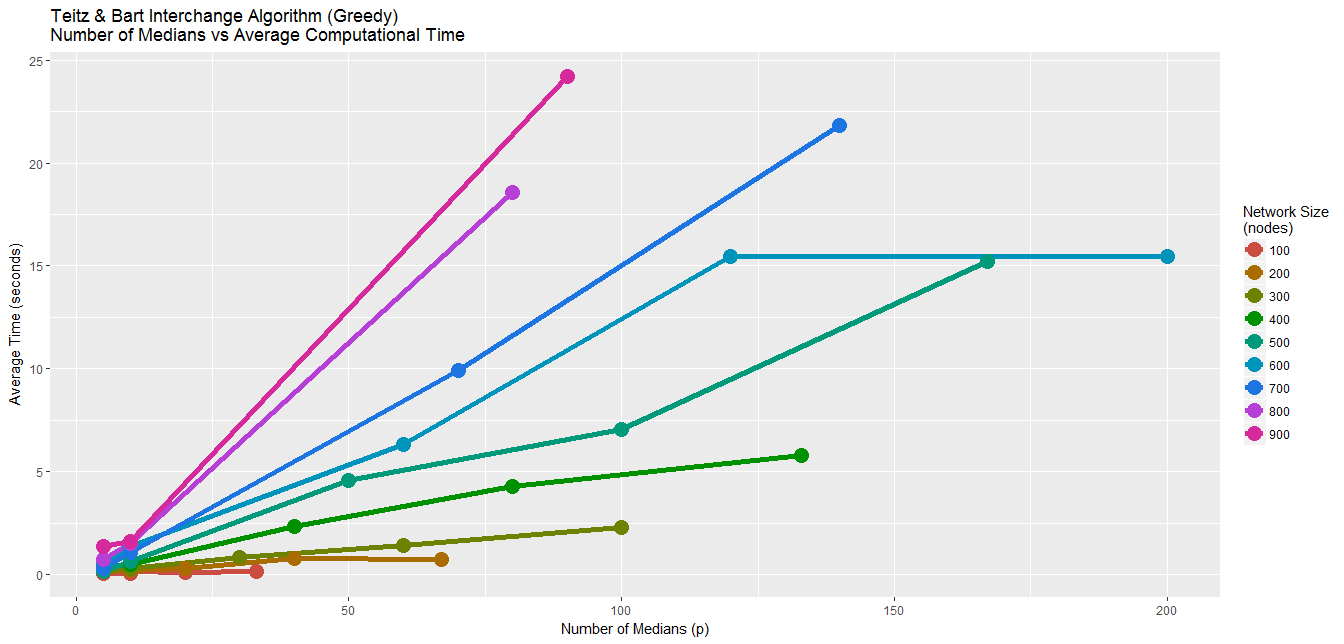
\includegraphics[width=15cm]{TBGreedy.png}
			\caption{Interchange Algorithm of Teitz and Bart with a Greedy Starting Solution}
			\label{TBGreedy.median.time}
		\end{center}
	\end{figure}

	Figure \ref{TBRand.median.time} shows the average computational time taken to produce the final result by the Teitz and Bart algorithm \index[terms]{interchange algorithm of Teitz and Bart}\index[terms]{interchange algorithm of Teitz and Bart! results}\index[terms]{local search heuristic!interchange algorithm of Teitz and Bart}\index[terms]{heuristic!interchange algorithm of Teitz and Bart} when presented with a solution that was produced by random feasible solution.  Clearly, more interchanges will be required before the algorithm finds a good solution and stops and as such, more time is required.  This can be seen in the bigger spread in computational time for the $p=5$ test problems.

	\begin{figure}[H]
	\begin{center}
		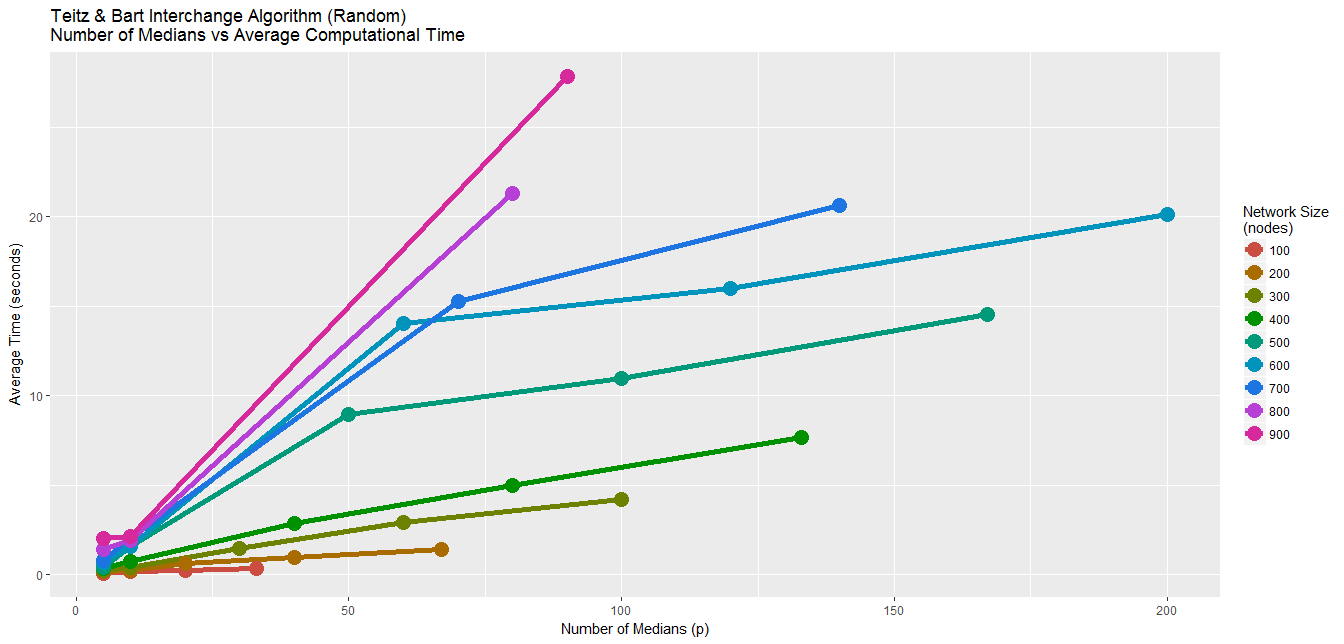
\includegraphics[width=15cm]{TBRand.png}
		\caption{Interchange Algorithm of Teitz and Bart with a Random Starting Solution}
		\label{TBRand.median.time}
	\end{center}
	\end{figure}

	Generally, using a greedy starting solution does result in some computational time savings during the local search when compared to using a random solution.  However, there are some exceptions with test problems 25, 29, and 30.  These three problems have large networks and demand a high number of medians.
	
	\subsection{The Fast Interchange Algorithm} \label{fastintalgo}
	The fast interchange algorithm,\index[terms]{heuristic!fast interchange}\index[terms]{fast interchange}\index[terms]{local search} proposed by Whitaker\index[author]{Whitaker, R.} \cite{WHIT83}, is based on the Teitz and Bart algorithm\index[terms]{heuristic!interchange algorithm of Teitz and Bart}\index[terms]{interchange algorithm of Teitz and Bart}  from subsection \ref{tbalgo}.  When searching for a free node that should be swapped with a node in the median set, only free nodes that have yet to be examined are considered.
	
	\subsubsection{Pseudocode}
	\index[terms]{fast interchange! pseudocode} 	
	\begin{algorithm}
		\caption{Fast Interchange Algorithm}
		\begin{algorithmic}[0]
			\Statex 
			\Statex INPUT: Cost Matrix; $P^*$; $S^*$
			
			\Statex 
			\Statex STEP 0: Initialisation
			\begin{equation*}
			\text{Set } k = z = q = 1 \text{ and } b=m-p
			\end{equation*}
			\begin{equation*}
			\text{Define } P=M-P^*
			\end{equation*}
			\Statex For each node in the network, determine the distance to both the closest node in the median set as well as the second closest node in the median set.
			\Statex For $i=1,2,\dots,n ,$ find \emph{x} and \emph{y} where \emph{x}, $y \in P^*$ such that
			\begin{align*}
			u_i^1 & = d_{ix} = \min_{j\in P^*}d_{ij}\\
			w_i^1 & = d_{iy} = \min_{j\in P^*, j\neq x}d_{ij}
			\end{align*}

			
			\Statex
			\Statex STEP 1: Calculate the change in the objective function if one node from the median set were to be interchanged with a free node.
			\Statex Set $r=P_q$ and find some node \emph{t}, $t \in P^*$ such that
			\begin{align*}
			S_{rt} &= \bigg[\sum_{i \in I}d_{ir}-u_i^k\bigg] + \min_{j\in P^*}\bigg[\sum_{i \in K_j}[\min(d_{ir}, w_i^k)-u_i^k]\bigg]\\
			\text{where } I &= \{\text{all } i \in G: d_{ir}<u_i^k\}\\
			\text{and } K_j &= \{\text{all } i \in G: d_{ir}\geq u_i^k\text{ and } d_{ij} - u_i^k\}
			\end{align*}

\Statex	
\algstore{fintbreak}
\end{algorithmic}
\end{algorithm}


\begin{algorithm}
\begin{algorithmic}[0]
\algrestore{fintbreak}


			\Statex
			\Statex STEP 2: If the objective function value were to increase by the proposed interchange of nodes, then go to STEP 4.  If the proposed change of nodes results in a decrease of the objective function value, then make the change, update iterative parameters and the objective function and go to STEP 3.
			\If{$S_{rt} \geq 0$}
			\Statex go to STEP 4
			[
			\ElsIf{$S_{rt} < 0$}
			\begin{equation*}
			k = k+1 \quad  S^*= S* + S_{rt} \quad P_q = \{t\} \quad P^*= P^*\backslash \{t\} \cup \{r\} \text{ and  go to STEP 3}
			\end{equation*}				
			]
			\EndIf


			\Statex
			\Statex STEP 3: Update the cost of travel for each node in the network to the closest and second closest medians.
			\If{$d_{it} > u_i^{k-1}$}
			\begin{align*}
			u_i^k & = \min(d_{ir},u_k^{k-1})
			\end{align*}
			\Statex let $s \in P^*$ be a median for node $i$ such that $d_{is} = u_i^k$
			\begin{align*}
			\text{set } w_i^k & = u_i^{k-1} \text{ if } d_{ir} \leq u_i^{k-1}\\
			\text{or set } w_i^k & = \min(d_{ir},w_i^{k-1}) \text{ if } d_{ir} > u_i^{k-1} \text{ and } d_{it} > w_i^{k-1}\\
			\text{or set } w_i^k & = \min_{j\in P^*,j\neq s}d_{ij} \text{ if } d_{ir} > u_i^{k-1} \text{ and } d_{it} = w_i^{k-1}
			\end{align*}
			[
			\ElsIf{$d_{it}=u_i^{k-1}$}
			\begin{align*}
			u_i^k & = \min(d_{ir},w_k^{k-1})
			\end{align*}
			\Statex let $s \in P^*$ be a median for node $i$ such that $d_{is} = u_i^k$
			\begin{equation*}
			\text{set } w_i^k  = w_i^{k-1} \text{ if } d_{ir} \leq w_i^{k-1}
			\text{ or set } w_i^k = \min_{j\in P^*,j\neq s}d_{ij} \text{ if }d_{ir} > w_i^{k-1}
			\end{equation*}
			]
			\EndIf			
			
\Statex	
\algstore{fintbreak}
\end{algorithmic}
\end{algorithm}


\begin{algorithm}
\begin{algorithmic}[0]
\algrestore{fintbreak}
			
			\Statex
			\Statex STEP 4: Once the algorithm has assessed all free nodes, go to STEP 5. Otherwise, increase the iterative parameters and go back to STEP 1.
			\If{$z=b$}
			\Statex go to STEP 5
			[
			\ElsIf{$z < b$}
			\begin{equation*}
			z=z+1 \text{, } q=q+1 \text{ and go to STEP 1}
			\end{equation*}
			]
			\EndIf

			
			\Statex
			\Statex STEP 5: If the algorithm finds that the current median set cannot be improved upon, then find the percent of free nodes that were assessed for a possible exchange from the free node set to the median set and stop.
			\begin{center}
				$a=\frac{q}{b}$ and STOP
			\end{center}
			
		\end{algorithmic}
	\end{algorithm}

	\subsubsection{Results}
	Table \ref{FI.Results.table} presents the average solution accuracy and the average computational time for the fast interchange algorithm.\index[terms]{heuristic!fast interchange}\index[terms]{fast interchange}\index[terms]{fast interchange!results}\index[terms]{local search}  The results from using a solution obtained from the greedy algorithm given in section \ref{classicheuristics.constructive} as well as a randomly created feasible solution are provided alongside one another for comparison.
	
	A comparison of the number of required medians versus the average computational time is given in figure \ref{FintGreedy.median.time} for a greedy starting solution and in figure \ref{FintRand.median.time} for a random staring solution.  Once again, when the algorithm was presented with a good solution it was quicker to find a final answer.  It can also be seen that as the size of the network and required number of medians increases, so does the computational time required by the algorithm.
	
	Figure \ref{FintGreedy.median.time} and figure \ref{FintRand.median.time} are very similar, but when the algorithm is presented with a random solution, it does take longer for every test problem.  Generally, the larger the number of nodes in the network along with the higher the number of required medians, the bigger the difference in time between the greedy solution and the random solution with the biggest difference occurring in test problem 30 which has the highest value of $p$ out of all the forty test problems.  When given the greedy solution for test problem 30, the fast interchange completed after 21.16 seconds compared to the 24.51 seconds for the random solution.
	
	\begin{figure}[H]
		\begin{center}
			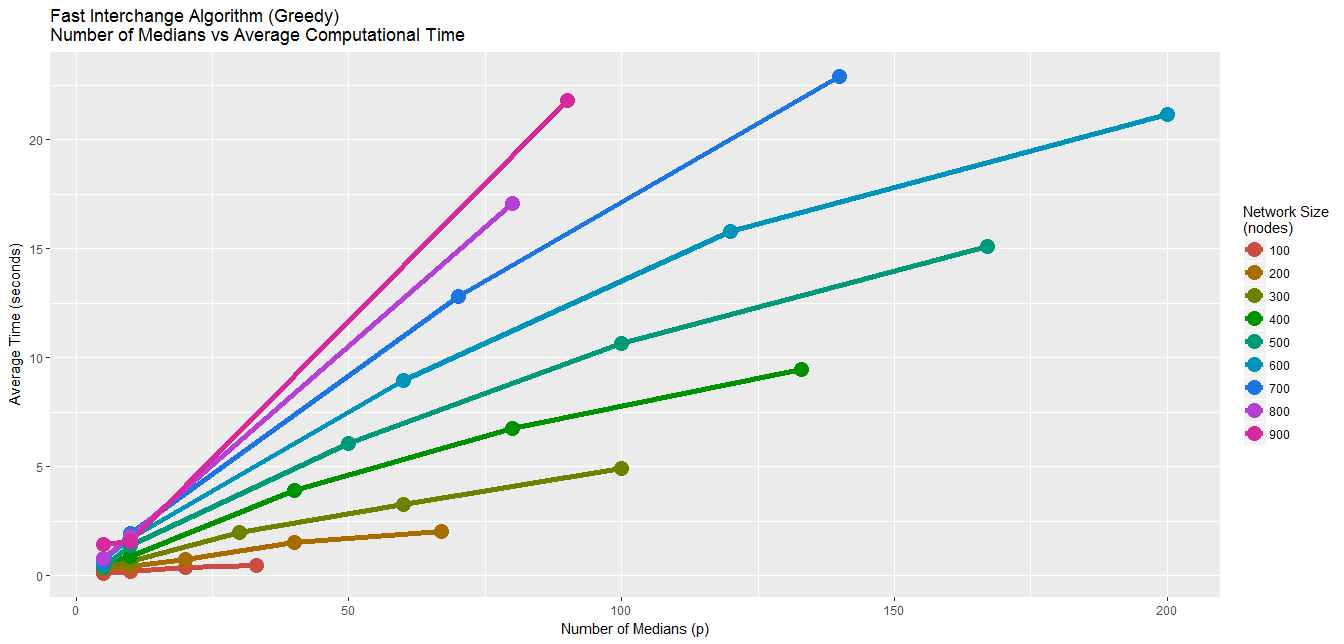
\includegraphics[width=15cm]{FintGreedy.png}
			\caption{Fast Interchange Algorithm with a Greedy Starting Solution}
			\label{FintGreedy.median.time}
		\end{center}
	\end{figure}
	
	\begin{figure}[H]
		\begin{center}
			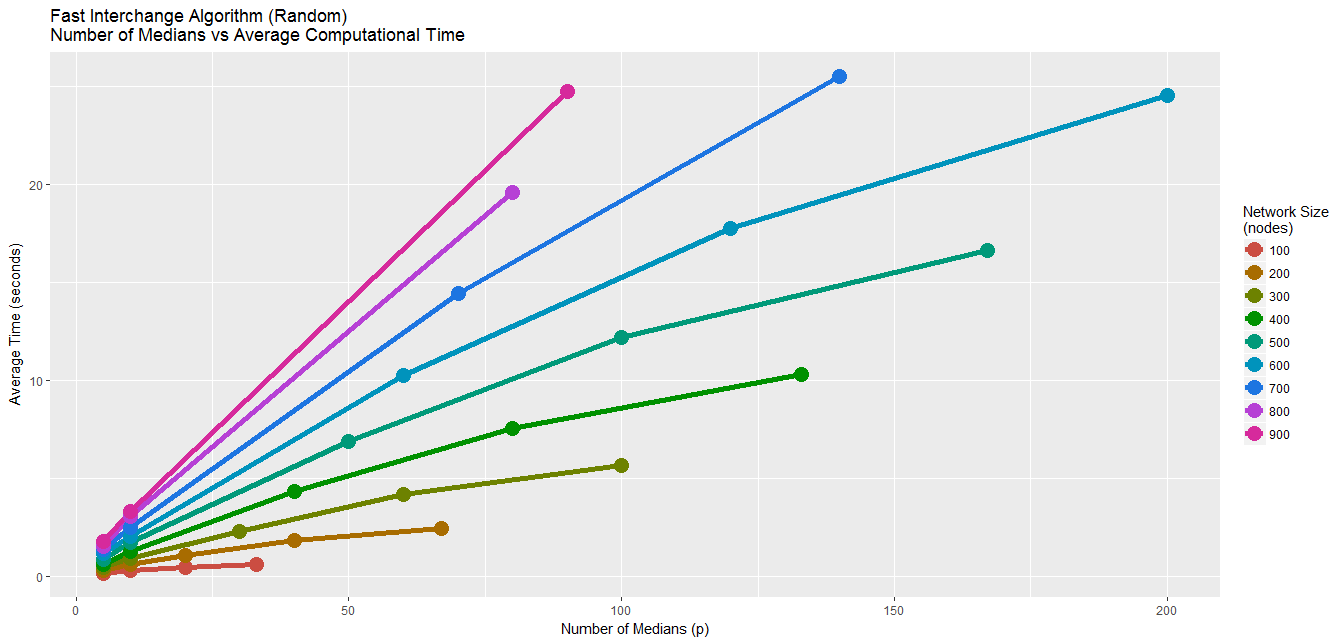
\includegraphics[width=15cm]{FintRand.png}
			\caption{Fast Interchange Algorithm with a Random Starting Solution}
			\label{FintRand.median.time}
		\end{center}
	\end{figure}

	Once again, this algorithm does not live up to its name with the fast interchange algorithm producing results faster than the interchange of Teitz and Bart on only four occasions.  As such, the design and code of this algorithm needs to be reviewed in order to see where possible savings can be found.

	\begin{table}[]
		\centering
		\caption{Local Search Heuristic Results - Fast Interchange Algorithm}
		\index[terms]{heuristic!fast interchange}\index[terms]{fast interchange}\index[terms]{fast interchange!results}
		\label{FI.Results.table}
		\begin{tabular}{ccccccc}
			\hline
			&  &  & \multicolumn{2}{c}{\textbf{GREEDY}} & \multicolumn{2}{c}{\textbf{RANDOM}} \\ \cline{4-7} 
			\multirow{-2}{*}{\textbf{\begin{tabular}[c]{@{}c@{}}\small{Test} \\ \small{Problem}\end{tabular}}} & \multirow{-2}{*}{\textbf{\begin{tabular}[c]{@{}c@{}}\small{Medians} \\ \small{(p)}\end{tabular}}} & \multirow{-2}{*}{\textbf{\begin{tabular}[c]{@{}c@{}}\small{Network} \\ \small{(nodes)}\end{tabular}}} & \textbf{\begin{tabular}[c]{@{}c@{}}\small{Av. Sol.}\\ \small{Accuracy}\end{tabular}} & \textbf{\begin{tabular}[c]{@{}c@{}}\small{Av. Comp.} \\ \small{Time (sec)}\end{tabular}} & \textbf{\begin{tabular}[c]{@{}c@{}}\small{Av. Sol.}\\ \small{Accuracy}\end{tabular}} & \textbf{\begin{tabular}[c]{@{}c@{}}\small{Av. Comp.}\\ \small{Time (sec)}\end{tabular}} \\ \hline
			\rowcolor[HTML]{EFEFEF} 
			01 & 5 & 100 & 1.00 & 0.11 & 1.00 & 0.16 \\
			\rowcolor[HTML]{EFEFEF} 
			02 & 10 & 100 & 1.00 & 0.16 & 1.00 & 0.29 \\
			\rowcolor[HTML]{EFEFEF} 
			03 & 10 & 100 & 1.00 & 0.19 & 0.97 & 0.28 \\
			\rowcolor[HTML]{EFEFEF} 
			04 & 20 & 100 & 1.00 & 0.37 & 0.99 & 0.44 \\
			\rowcolor[HTML]{EFEFEF} 
			05 & 33 & 100 & 1.00 & 0.45 & 0.97 & 0.61 \\
			06 & 5 & 200 & 1.00 & 0.27 & 1.00 & 0.30 \\
			07 & 10 & 200 & 1.00 & 0.40 & 1.00 & 0.60 \\
			08 & 20 & 200 & 1.00 & 0.71 & 1.00 & 1.06 \\
			09 & 40 & 200 & 0.99 & 1.52 & 0.99 & 1.81 \\
			10 & 67 & 200 & 0.99 & 2.00 & 0.98 & 2.45 \\
			\rowcolor[HTML]{EFEFEF} 
			11 & 5 & 300 & 1.00 & 0.36 & 1.00 & 0.44 \\
			\rowcolor[HTML]{EFEFEF} 
			12 & 10 & 300 & 1.00 & 0.62 & 1.00 & 0.92 \\
			\rowcolor[HTML]{EFEFEF} 
			13 & 30 & 300 & 1.00 & 1.99 & 0.99 & 2.30 \\
			\rowcolor[HTML]{EFEFEF} 
			14 & 60 & 300 & 1.00 & 3.24 & 0.99 & 4.18 \\
			\rowcolor[HTML]{EFEFEF} 
			15 & 100 & 300 & 0.99 & 4.93 & 0.97 & 5.64 \\
			16 & 5 & 400 & 1.00 & 0.58 & 1.00 & 0.58 \\
			17 & 10 & 400 & 1.00 & 0.86 & 1.00 & 1.26 \\
			18 & 40 & 400 & 1.00 & 3.89 & 1.00 & 4.31 \\
			19 & 80 & 400 & 0.99 & 6.76 & 0.99 & 7.56 \\
			20 & 133 & 400 & 0.99 & 9.44 & 0.97 & 10.31 \\
			\rowcolor[HTML]{EFEFEF} 
			21 & 5 & 500 & 1.00 & 0.38 & 1.00 & 0.86 \\
			\rowcolor[HTML]{EFEFEF} 
			22 & 10 & 500 & 0.99 & 1.37 & 0.99 & 1.72 \\
			\rowcolor[HTML]{EFEFEF} 
			23 & 50 & 500 & 1.00 & 6.06 & 0.99 & 6.89 \\
			\rowcolor[HTML]{EFEFEF} 
			24 & 100 & 500 & 1.00 & 10.66 & 0.99 & 12.19 \\
			\rowcolor[HTML]{EFEFEF} 
			25 & 167 & 500 & 0.99 & 15.12 & 0.98 & 16.59 \\
			26 & 5 & 600 & 1.00 & 0.76 & 1.00 & 1.15 \\
			27 & 10 & 600 & 1.00 & 1.68 & 1.00 & 2.05 \\
			28 & 60 & 600 & 1.00 & 8.95 & 0.99 & 10.24 \\
			29 & 120 & 600 & 1.00 & 15.80 & 0.99 & 17.73 \\
			30 & 200 & 600 & 0.99 & 21.16 & 0.98 & 24.51 \\
			\rowcolor[HTML]{EFEFEF} 
			31 & 5 & 700 & 1.00 & 0.57 & 1.00 & 1.35 \\
			\rowcolor[HTML]{EFEFEF} 
			32 & 10 & 700 & 1.00 & 1.93 & 1.00 & 2.49 \\
			\rowcolor[HTML]{EFEFEF} 
			33 & 70 & 700 & 0.99 & 12.82 & 0.99 & 14.42 \\
			\rowcolor[HTML]{EFEFEF} 
			34 & 140 & 700 & 0.99 & 22.89 & 0.99 & 25.48 \\
			35 & 5 & 800 & 1.00 & 0.78 & 1.00 & 1.50 \\
			36 & 10 & 800 & 1.00 & 1.79 & 1.00 & 3.05 \\
			37 & 80 & 800 & 1.00 & 17.07 & 0.99 & 19.58 \\
			\rowcolor[HTML]{EFEFEF} 
			38 & 5 & 900 & 0.99 & 1.43 & 0.99 & 1.79 \\
			\rowcolor[HTML]{EFEFEF} 
			39 & 10 & 900 & 1.00 & 1.56 & 1.00 & 3.28 \\
			\rowcolor[HTML]{EFEFEF} 
			40 & 90 & 900 & 1.00 & 21.83 & 0.99 & 24.73
		\end{tabular}
	\end{table}
	
	
	\subsection{The Alternate Algorithm} \label{alternatealgo}
	The alternate algorithm\index[terms]{heuristic!alternate algorithm}\index[terms]{alternate algorithm}\index[terms]{local search} was presented in a paper by Maranzana \index[author]{Maranzana, F.} in 1964 \cite{MARA64} and begins with creating a random median set and assigning all nodes in the network to one of these median nodes.  The group of free nodes associated with each median node is evaluated and the median for this group is determined and replaces the node in the median set if different from the current median.  All nodes in the network are then reassigned to the closest median in the new median set and once again each group's true median is determined and replaces the current node in the median set.  This process continues until there is an iteration with no changes to the median set.
	
	\subsubsection{Pseudocode}
	\index[terms]{alternate! pseudocode} 	
	\begin{algorithm}
		\caption{Alternate Algorithm}
		\begin{algorithmic}[0]
			\Statex 
			\Statex INPUT: Cost Matrix; $P^*$; $S^*$
			
			\Statex 
			\Statex STEP 0: Initialisation
			\Statex Randomly assign $p$ nodes to $P^*$ and set $P = M - P^*$
			
			\Statex 
			\Statex STEP 1: Assign each node in the network to its closest median.
			\begin{align*}
			K_j=\{\text{all } i \in G \text{ such that } \min (d_{ij})\} \text{ where } j \in P^*
			\end{align*}
			
			\Statex 
			\Statex STEP 2: Find the median node for each current median's set of associated nodes.
			\begin{equation*}
			\text{Find } k_j \in K_j \text{ where } \min \bigg[ \sum_{i\in K_j} d_{ik} \bigg] 
			\end{equation*}
			
			
			\Statex 
			\Statex STEP 3: Update $P^*$ with the new set of medians.
			\begin{equation*}
			P^{*} = \{\text{all } k_j  \} \text{ for } j \in P^*
			\end{equation*}
			
			
		\end{algorithmic}
	\end{algorithm}

	\subsubsection{Results}
	The code for this algorithm has not been completed and as such there are no results that can be presented at this time.
	
	\subsection{Computational Results} \label{classicheuristics.localsearch.results}
	Figure \ref{LS.av.acc} shows the average accuracy of the objective function value obtained from the two algorithms that were run for both of the different starting solutions.  The results fluctuate between returning a result that is 3\% worse than the optimal and the perfect solution.  The fast interchange algorithm using a random starting solution produced the most variation.  It is the fast interchange with a random starting solution that results in the greatest variation in accuracy, while the fast interchange\index[terms]{heuristic!fast interchange}\index[terms]{fast interchange}\index[terms]{fast interchange!results} with a greedy solution along with both variations in the interchange algorithm of Teitz and Bart\index[terms]{heuristic!interchange algorithm of Teitz and Bart}\index[terms]{interchange algorithm of Teitz and Bart}\index[terms]{interchange algorithm of Teitz and Bart! results} produce consistently accurate results.
	
	\begin{figure}[H]
		\begin{center}
			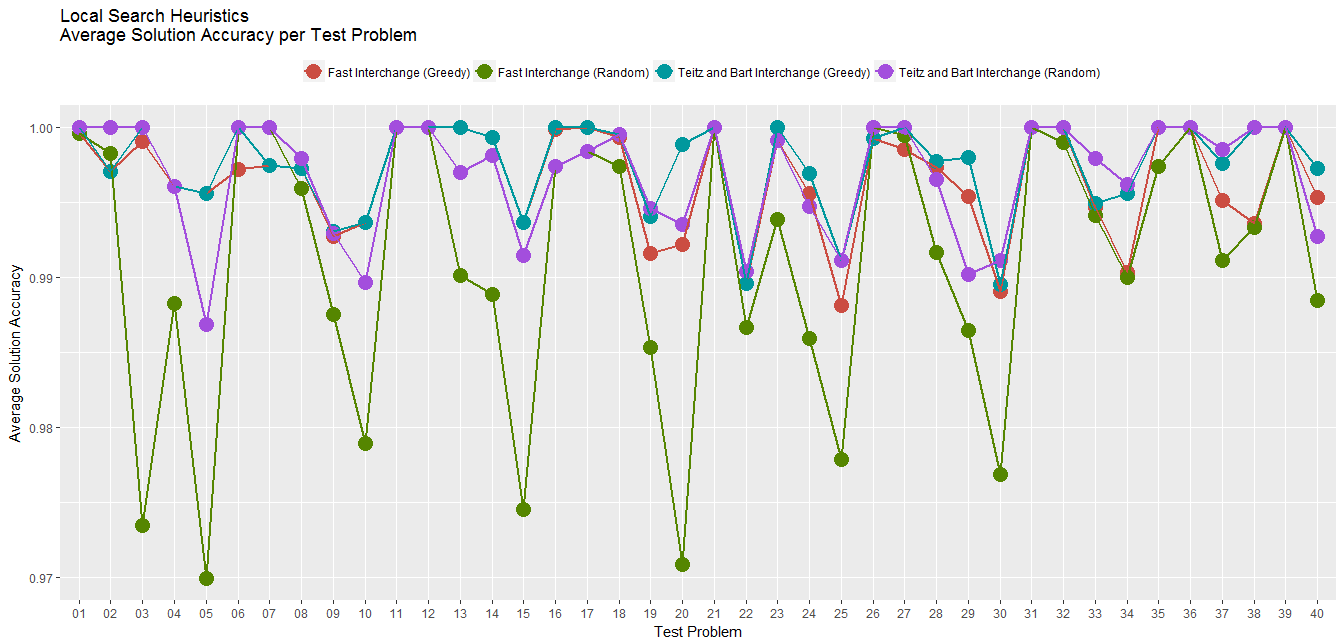
\includegraphics[width=14cm]{LSavacc.png}
			\caption{Average Solution Accuracy per Test Problem}
			\label{LS.av.acc}
		\end{center}
	\end{figure}

	The average computational time required by the two algorithms shows similar results to that of the constructive greedy algorithm when the value of $p$ is small, but as the network size increases along with the value of $p$, the computational time increases dramatically.


	\begin{figure}[H]
		\begin{center}
			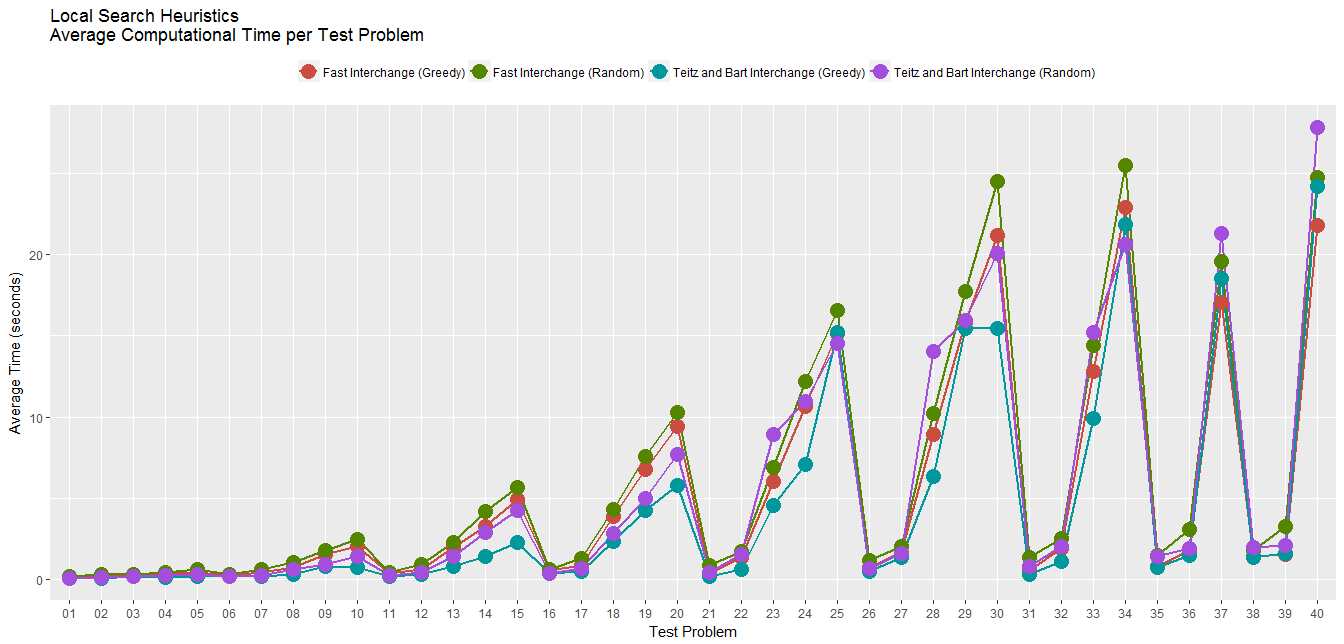
\includegraphics[width=14cm]{LSavtime.png}
			\caption{Average Computational per Test Problem}
			\label{LS.av.time}
		\end{center}
	\end{figure}

		
	\section{Conclusion} \label{conclusion}
	The results from the local search heuristics offer only a small improvement on those produced by the constructive greedy algorithm from section \ref{classicheuristics.constructive} as that algorithm produced solutions that were up to 4\% worse than the optimal value.  The increase in time between the constructive greedy algorithm and the local search algorithms are significantly large particularly for larger networks that require a lot of medians.  Test problem 30 took just over 2 seconds to produce a solution that was on average 97\% accurate while the interchange algorithm of Teitz and Bart and the fast interchange algorithm both improved this accuracy by 2\%, but at a cost of an additional 13 and 19 seconds respectively.  Of course, context is king and for many real-world problems a 2\% improvement could equate to vast amounts of savings and as such this small improvement may be worth the additional computational time that is required.
	
	Looking at the difference in time between both local search algorithms starting with a random solution and a greedy solution, it can be seen that the additional time taken to improve the random solution is generally greater than the time taken by the greedy algorithm to find a starting solution.
	
	
	\section{Remaining Work}
	In the coming weeks, the literature study in section \ref{lit.study} will be extended to give more background into the algorithms investigated in this study and the section giving an overview of heuristics may also be broadened.
	
	Of the six algorithms currently included in this study, only the alternate algorithm needs to coded.  This will be done and the results from running this code will be added to the local search computational results.  The stingy algorithm code has been completed, but needs to be revised as the computational time required for even small problems is excessively high.  The results from this algorithm will also be included and analysed, even if code cannot be improved.
	
	The complexity of all the algorithms will be added to their respective subsections and may be referred to in the subsection comparing the results if appropriate.
	
	As has already been mentioned, the fast greedy algorithm and the fast interchange algorithm are taking longer to run than the original algorithm.  This goes against what was expected and the reason that this is occurring needs to be determined.  Current thoughts are that algorithm code could be improved as well as the fact that the design R language is able to determine the closest median for all nodes in the network a computationally inexpensive which makes the proposed improvements offered by the two "fast" algorithms redundant.  R code can be profiled to determine where bottlenecks slowing down the processing time exist and from this information, hopefully, the code can be improved.  Vectorisation is a key component of the R language as it allows for an increase in speed.  It is currently not known if this has been fully exploited in the code that has been written for this study and as such this needs to be assessed and applied.
	
	Given time, a section on metaheuristics used to solve the $p$-median problem will also be added.  At least two metaheuristics will be coded and used to solve the forty test problems.  These results will also be added to the final report and compared to those produced in the classic heuristic sections.
		
		
	\np
	\bibliography{finalbib}
	\bibliographystyle{IEEEtran}
	\np

	\printindex[terms]
	\printindex[authors]
	


\end{document}